\input{head.inc}
  
% Präambelbefehle für die Präsentation
\title[TET: Quasistationäre Felder III- Felddiffusion im Halbraum]{Quasistationäre Felder III - Felddiffusion im Halbraum}

\begin{document}
% 
% Frontmatter 
% 
%%%%%%%%%%%%%%%%%%%%%%%%%%%%%%%%%%%%%%%%%%%%%%%%%%%%%%%%%%%%%%%%%%%%%%%%%%%%%%%%%%%%%%%%%%%%%%%%%%%%%%%%%%%%%%%%%%%%%%%%%%%%% 

%% inserts the title page and the table of contents
\maketitle

% 
% Content 
% 
%%%%%%%%%%%%%%%%%%%%%%%%%%%%%%%%%%%%%%%%%%%%%%%%%%%%%%%%%%%%%%%%%%%%%%%%%%%%%%%%%%%%%%%%%%%%%%%%%%%%%%%%%%%%%%%%%%%%%%%%%%%%% 
\section{Quasistationäre Felder III - Felddiffusion im Halbraum}

\begin{frame}
  \frametitle{Problemstellung}
  \begin{columns}
    \begin{column}{.4\linewidth}
      \centerline{\resizebox{\columnwidth}{!}{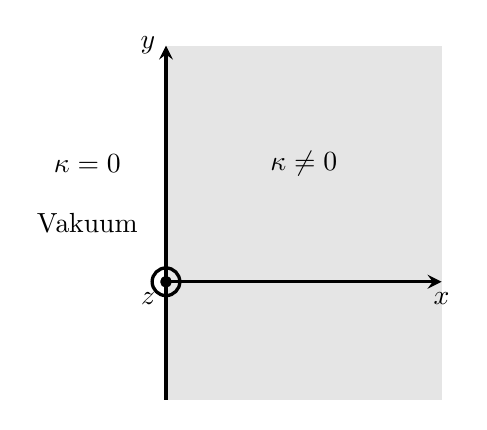
\begin{tikzpicture}[line width = 1.2pt, line join=round,x=1cm,y=1cm,>=stealth]
	% Schatten für den Stoff
	\fill [color = lightgray!40] (0,3) rectangle (3.5,-1.5);
	% Koordinatensystem
	\draw [->] (0,0) -- (3.5,0) node [anchor = north] {$ x $};
	\draw [->] (0,-1.5) -- (0,3) node [anchor = east] {$ y $};
	\filldraw (0,0) circle (1.5pt);
	\draw (0,0) circle (5pt);
	\draw (0,0) node [anchor = north east] {$ z $};
	% Leitfähigkeiten
	\draw (1.75,1.5) node {$ \kappa \neq 0 $};
	\draw (-1,1.5) node {$ \kappa = 0 $};
	\draw (-1,0.75) node {Vakuum};
\end{tikzpicture}}}
      \end{column}
   \begin{column}{.6\linewidth}
  \begin{itemize}[<+->]
  \item Zwei unendlich ausgedehnten Halbräume (Vakuum und Leiter) $\to$ translationsinvarianz in $y$ und $z$- Richtung
  \item \(\EFeld[v] \) und \(\BFeld[v] \) unabhängig von \(y\) und \(z\)
\item Ableitungen nach \(y\) und \(z\) sind Null
  $$
  \dfrac{\partial}{\partial y} = \dfrac{\partial}{\partial z} = 0
  $$
  \item Lösungsgebiet: $x>=0$ (im Leiter)
  \item harmonische Zeitabhängigkeit: $\frac{\partial}{\partial t} \to \komplex\omega$
  \end{itemize}
\end{column}
\end{columns}\pause

\begin{align*}
\laplace \EFeld[uv] &= \komplex\omega\mu\kappa \EFeld[uv]    & \laplace \BFeld[uv] &= \komplex \omega\mu \kappa \BFeld[uv]\\ 
\dfrac{\partial^2}{\partial x^2} \EFeld[uv] &= \komplex\omega\mu \kappa \EFeld[uv] & \dfrac{\partial^2}{\partial x^2} \BFeld[uv] &= \komplex \omega \mu \kappa \BFeld[uv]\\
\EFeld[uv] & = \sum_{i=x,y,z}\EFeld[u]_i \vu{i} & \BFeld[uv] &= \sum_{i=x,y,z}\BFeld[u]_i \vu{i}
\end{align*}
\end{frame}

\begin{frame}
  \frametitle{Bestimmungsgleichungen}
  \begin{itemize}[<+->]
  \item Rotation des E-Feldes hat keine x-Komponente. Es gilt:
$$
\rotation \EFeld[uv] = \varepsilon_{ijk} \vu{i} \partial_j\EFeld[u]_k \stackrel{\text{hier}}{=} -\partial_x\EFeld[u]_z \vu{y} + \partial_x\EFeld[u]_y \vu{z} \stackrel{!}{=} -\komplex\omega   \sum_{i=x,y,z}\BFeld[u]_i \vu{i} \to \boxed{\BFeld[u]_x=0}
$$
\item Analog: Rotation des B-Feldes (H-Feldes) hat keine x-Komponente. Damit folgt:
  $$
  \mu^{-1} \rotation\BFeld[uv] = \rotation \HFeld[uv] = \StromDichte[uv] = \kappa\EFeld[uv] \to \text{ E-Feld hat keine x-Komponente: } \boxed{\EFeld[u]_x=0} 
  $$
\item Hiermit folgen 4 strukturgleiche skalare Diffusionsgleichungen
 \begin{align*}
\dfrac{\partial^2}{\partial x^2} \EFeld[u]_y &= \komplex \omega \mu \kappa \EFeld[u]_y & \dfrac{\partial^2}{\partial x^2} \BFeld[u]_y &= \komplex \omega \mu \kappa \BFeld[u]_y \\
\dfrac{\partial^2}{\partial x^2} \EFeld[u]_z &= \komplex \omega \mu \kappa \EFeld[u]_z & \dfrac{\partial^2}{\partial x^2} \BFeld[u]_z &= \komplex \omega \mu \kappa \BFeld[u]_z 
 \end{align*}
\item Es reicht, eine der Gleichungen zu betrachten: $\dfrac{\partial^2}{\partial x^2} \EFeld[u]_y = \komplex \omega \mu \kappa \EFeld[u]_y$ \\
  Hinweis: Stetigkeit von $E_t$; \alert{wähle} $\vu{y} \parallel \StromDichte[uv](x=0) = \kappa\EFeld[uv](x=0)$
  \end{itemize}
\end{frame}


\begin{frame}
  \frametitle{Eindringtiefe - Skin-Tiefe - Allgemeine Lösung}
  \begin{itemize}[<+->]
  \item Wir betrachten: $\dfrac{\partial^2}{\partial x^2} \EFeld[u]_y = \komplex \omega \mu \kappa \EFeld[u]_y$
  \item Ansatz: $\EFeld[u]_\mathrm{y} = \underline{A} \euler^{k x} \text{ mit } [k] = \si{\per\metre} $
  \item Dies liefert: $k^2 = \komplex \omega \mu \kappa$
    \item Und somit:
$$
	k_{1/2} = \pm \dfrac{1 + \komplex}{\sqrt{2}} \sqrt{\omega \mu \kappa}
		= \pm \left( 1 + \komplex \right) \sqrt{\dfrac{\omega \mu \kappa}{2}}
		= \pm \dfrac{1 + \komplex}{\delta}
$$
\item Hierbei ist $\delta$ die \alert{Eindringtiefe} bzw. \alert{Skin-Tiefe}
  $$
  \boxed{ \delta = \sqrt{\dfrac{2}{\omega \mu \kappa}} } \quad [\delta] =\si{\metre}
  $$
\item Die allgemeine Lösung ist somit
  $$
  \boxed{\EFeld[u]_\mathrm{y} = \underline{A}_1 \euler^{\nicefrac{x}{\delta}} \euler^{\komplex \nicefrac{x}{\delta}} + \underline{A}_2  \euler^{-\nicefrac{x}{\delta}} \euler^{-\komplex \nicefrac{x}{\delta}} }
  $$
  \end{itemize}
\end{frame}

\begin{frame}
  \frametitle{Allgemeine Lösung}
  \begin{itemize}[<+->]
\item gefundene Lösung: $\EFeld[u]_\mathrm{y} = \underline{A}_1 \euler^{\nicefrac{x}{\delta}} \euler^{\komplex \nicefrac{x}{\delta}} + \underline{A}_2  \euler^{-\nicefrac{x}{\delta}} \euler^{-\komplex \nicefrac{x}{\delta}} $
  \item Könnte analog auch für \(\EFeld[u]_z \), \(\BFeld[u]_y \) und \(\BFeld[u]_z \) hingeschrieben werden. Besser aber  $\rotation \EFeld[uv] = \varepsilon_{ijk} \vu{i} \partial_j\EFeld[u]_k = \textcolor{green}{-\partial_x\EFeld[u]_z \vu{y}} + \textcolor{red}{\partial_x\EFeld[u]_y \vu{z}} = -\komplex\omega   \sum_{i=x,\textcolor{green}{y},\textcolor{red}{z}}\BFeld[u]_i \vu{i}$:
\begin{align*}
\dfrac{\partial}{\partial x} \EFeld[u]_y &= -\komplex\omega\BFeld[u]_\mathrm{z} &\Rightarrow \BFeld[u]_z &= -\dfrac{1}{\komplex\omega} \dfrac{\partial}{\partial x} \EFeld[u]_y\\
&&& = -\dfrac{1 + \komplex}{\komplex \omega}  \dfrac{1}{\delta}  \left[ \underline{A}_1  \euler^{\nicefrac{x}{\delta}}  \euler^{\komplex \nicefrac{x}{\delta}} - \underline{A}_2 \euler^{-\nicefrac{x}{\delta}} \euler^{-\komplex \nicefrac{x}{\delta}} \right]
\end{align*}
\item Bestimmung der Konstanten
\begin{enumerate}[<+->]
 	\item Für \(x \,\rightarrow\, \infty \) muss das E-Feld verschwinden $\to$
$\boxed{\underline{A}_1 = 0}$
 	\item An der Oberfläche (\(x = 0 \)) gilt $\EFeld[u]_{y} = \EFeld[u]_{y}(x = 0) = \frac{1}{\kappa}\StromDichte[u]_y(x=0)=\EFeld[u]_{y0} =\frac{1}{\kappa}\StromDichte[u]_{y0}  \Rightarrow \boxed{\underline{A}_2 = \EFeld[u]_{y0}}$
        \end{enumerate}
\item Hiermit (o.B.d.A.: $\EFeld[u]_{z}(x = 0) = \EFeld[u]_{z0} = 0 \to$ andere Komponenten brauchen wir nicht) 
\begin{align*}
\EFeld[u]_{y} &= \EFeld[u]_{y0} \euler^{-\nicefrac{x}{\delta}} \euler^{-\komplex\nicefrac{x}{\delta}} & \HFeld[u]_\mathrm{z} &= \dfrac{\BFeld[u]_\mathrm{z}}{\mu} = \dfrac{1 + \komplex}{\komplex\omega\mu} \dfrac{1}{\delta} \EFeld[u]_{y0} \euler^{-\nicefrac{x}{\delta}} \euler^{-\komplex \nicefrac{x}{\delta}} & \delta &= \sqrt{\dfrac{2}{\omega \mu \kappa}}
\end{align*}
      \end{itemize}
\end{frame}


\begin{frame}
  \frametitle{Dämpfung - Phasendrehung}
  \begin{itemize}[<+->]
\item Ausgehend von 
\begin{align*}
\EFeld[u]_{y} &= \EFeld[u]_{y0} \euler^{-\nicefrac{x}{\delta}} \euler^{-\komplex\nicefrac{x}{\delta}} & \HFeld[u]_\mathrm{z} &= \dfrac{\BFeld[u]_\mathrm{z}}{\mu} = \dfrac{1 + \komplex}{\komplex\omega\mu} \dfrac{1}{\delta} \EFeld[u]_{y0} \euler^{-\nicefrac{x}{\delta}} \euler^{-\komplex \nicefrac{x}{\delta}} & \delta &= \sqrt{\dfrac{2}{\omega \mu \kappa}}
\end{align*}
\item stellen wir um:
\begin{align*}
\HFeld[u]_z &= \dfrac{1 - \komplex}{\omega \delta \mu} \EFeld[u]_{y0} \euler^{-\nicefrac{x}{\delta}} \euler^{-\komplex \nicefrac{x}{\delta}} \\
&= \left(1 - \komplex \right) \sqrt{\dfrac{\kappa}{2 \omega \mu}}  \EFeld[u]_{y0} \euler^{-\nicefrac{x}{\delta}} \euler^{-\komplex \nicefrac{x}{\delta}} \\
&= \dfrac{\kappa \delta}{2} \underbrace{\left( 1 - \komplex \right)}_{\sqrt{2}\euler^{-\komplex\nicefrac{\pi}{4}}} \EFeld[u]_{y0} \underbrace{\euler^{-\nicefrac{x}{\delta}}}_{\text{Dämpfung}} \underbrace{\euler^{-\komplex \nicefrac{x}{\delta}}}_{\substack{\text{Phasen-}\\ \text{drehung}}} = \underbrace{\kappa \EFeld[u]_{y0}}_{\StromDichte[u]_{y0}}\dfrac{\delta}{\sqrt{2}} \euler^{-\nicefrac{x}{\delta}} \euler^{-\komplex \nicefrac{x}{\delta}}\euler^{-\komplex\nicefrac{\pi}{4}}
\end{align*}
\item Es gilt: $\frac{\left| \HFeld[u]_{z}(x = \delta) \right|}{\left| \HFeld[u]_{z}(x = 0) \right|} = \frac{\left| \EFeld[u]_{y}(x = \delta) \right|}{\left| \EFeld[u]_{y}(x = 0) \right|}= \euler^{-1} \approx 0,37$; nach $2\delta$: $\euler^{-2} \approx 0,14$ usw.
      \end{itemize}
    \end{frame}
    
\begin{frame}
  \frametitle{Schwingungseigenschaften der Lösung}
  \href{https://bildungsportal.sachsen.de/opal/auth/RepositoryEntry/27455913992/CourseNode/103138906469436/Theoretische\%20Elektrotechnik/Quasistationäre\%20Felder/ey_hz.mp4}{$\to$ Video Link}
  \bigskip
  
  \centering
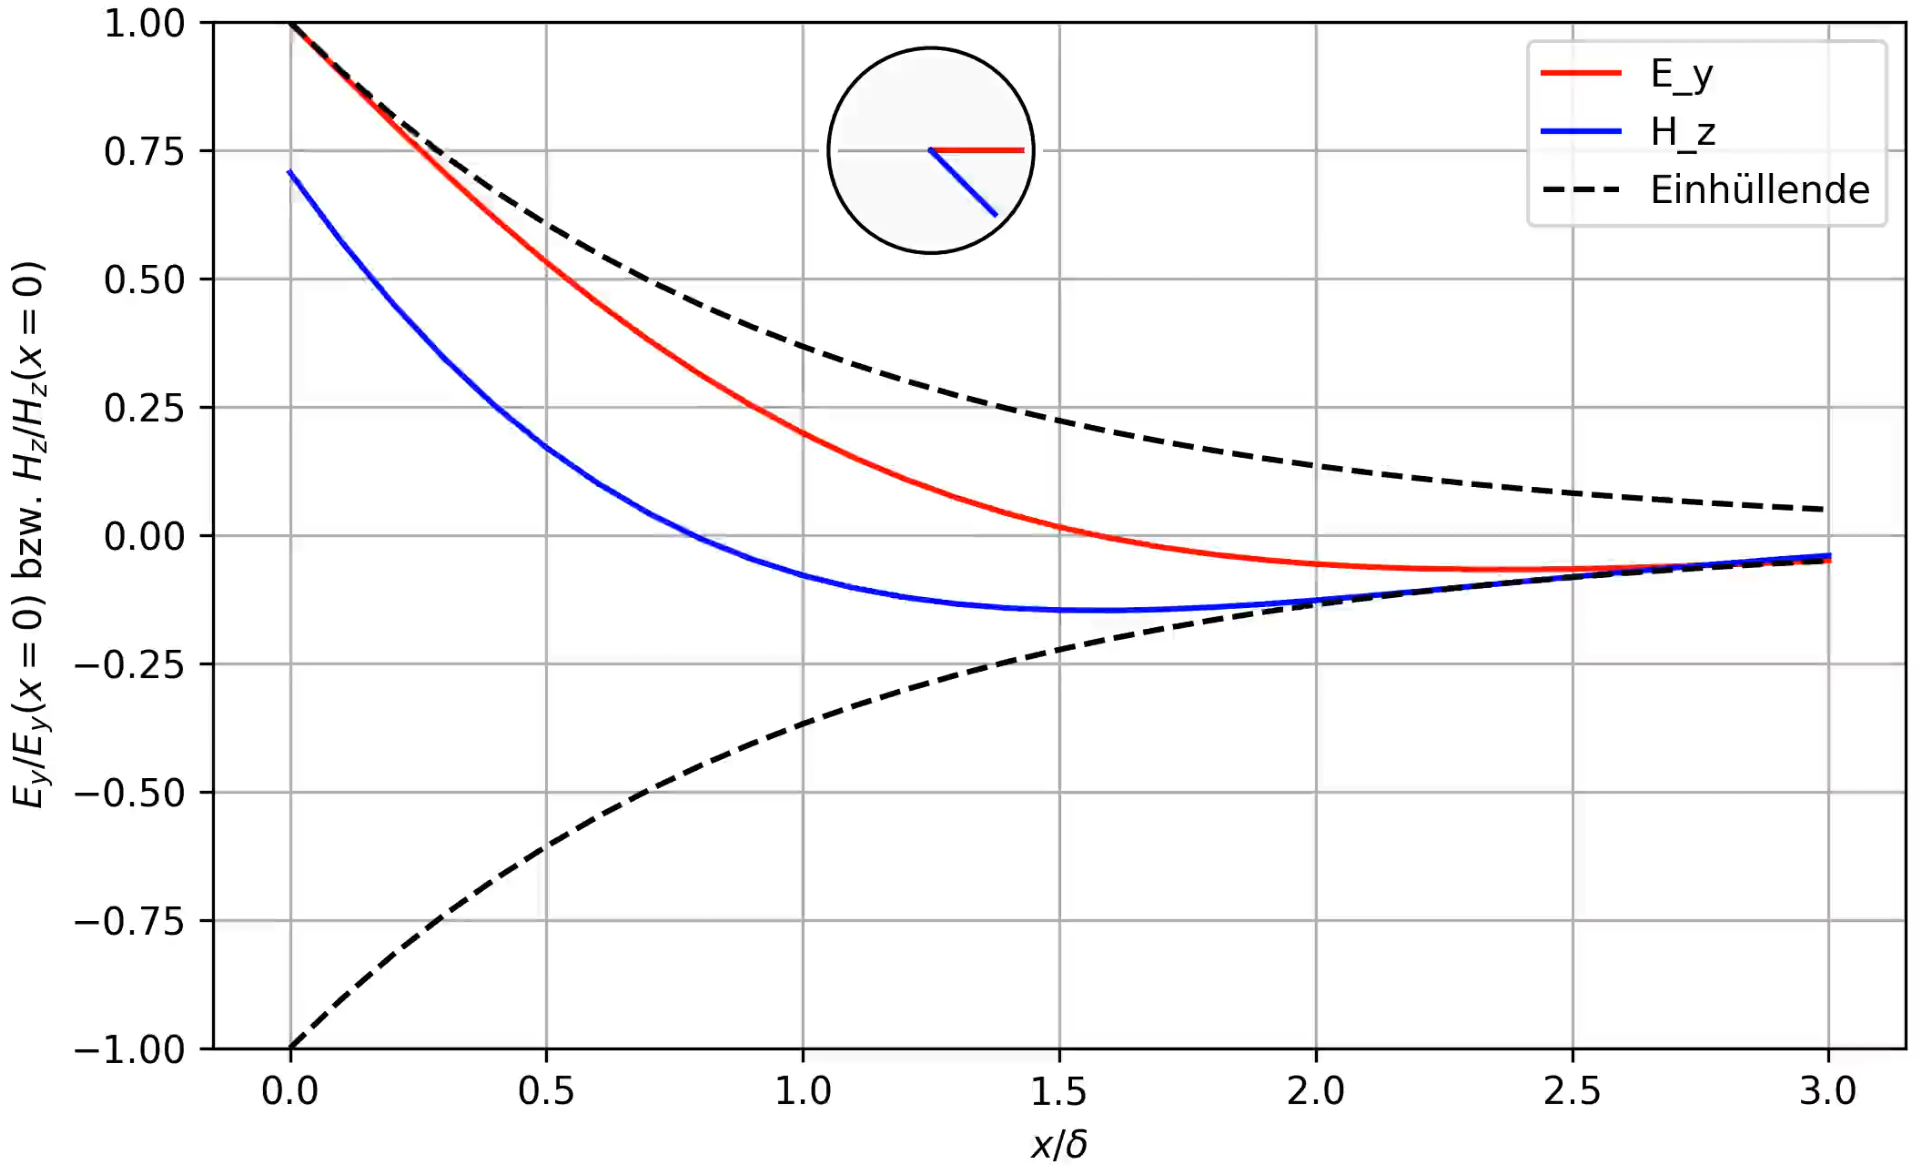
\includegraphics[width=.95\linewidth]{programs/Skin-Effect/ey_hz.png}
\end{frame}


\begin{frame}
  \frametitle{Eindringtiefe}
  \centering
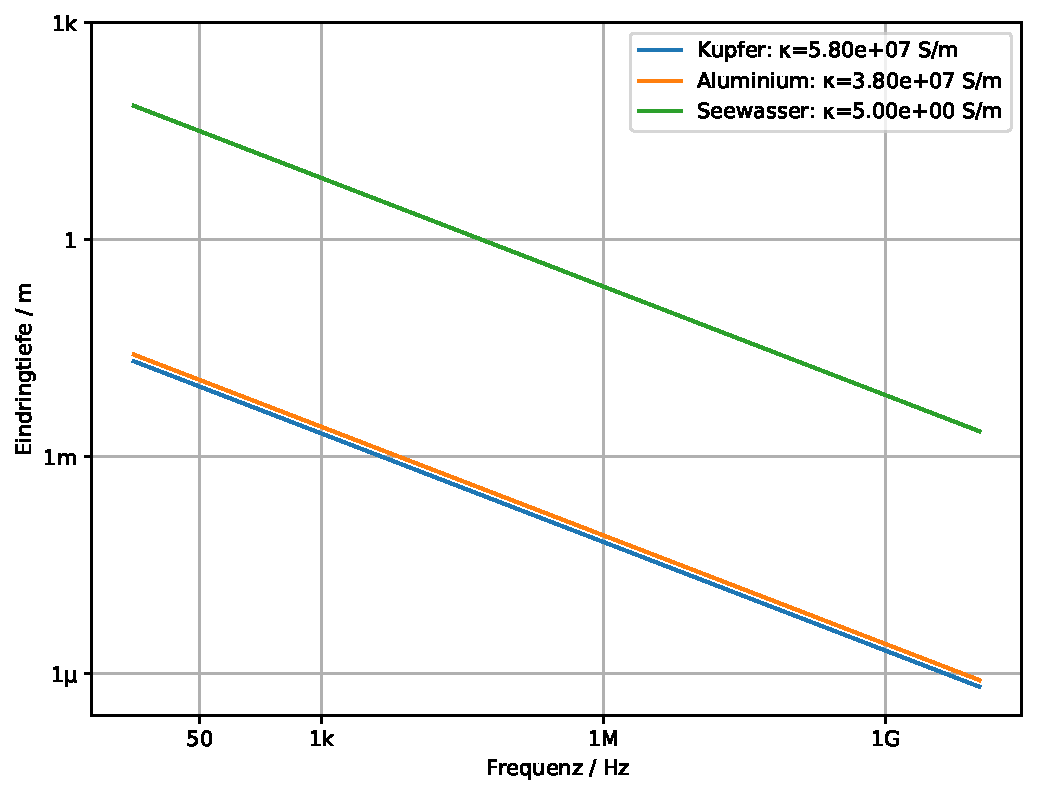
\includegraphics[width=.85\linewidth]{programs/Skin-Effect/skin_depth.pdf}
\end{frame}

\begin{frame}
  \frametitle{Lösung vor dem Leiter}
  \begin{itemize}[<+->]
\item Lösung für $x\ge 0$ (im Leiter): 
\begin{align*}
  \EFeld[uv] = \EFeld[u]_{y}\vu{y} &= \EFeld[u]_{y0} \euler^{-\nicefrac{x}{\delta}} \euler^{-\komplex\nicefrac{x}{\delta}}\vu{y} & \HFeld[uv] =\HFeld[u]_{z}\vu{z} &= \kappa \EFeld[u]_{y0}\dfrac{\delta}{\sqrt{2}} \euler^{-\nicefrac{x}{\delta}} \euler^{-\komplex \nicefrac{x}{\delta}}\euler^{-\komplex\nicefrac{\pi}{4}}\vu{z} \\
  \StromDichte[uv] = \StromDichte[u]_{y}\vu{y}=\kappa\EFeld[u]_{y}\vu{y} &= \kappa \EFeld[u]_{y0} \euler^{-\nicefrac{x}{\delta}} \euler^{-\komplex\nicefrac{x}{\delta}}\vu{y} & \delta &= \sqrt{\dfrac{2}{\omega \mu \kappa}}
\end{align*}
\item Berechnung des Magnetfeldes für $x<0$ (vor dem Leiter) über $\rotation \HFeld[v] = \StromDichte[v]$
  \begin{columns}
    \begin{column}{.4\linewidth}
      \resizebox{\columnwidth}{!}{\incfig{skin-H-Weg}}
    \end{column}
    \begin{column}{.6\linewidth}
      \begin{align*}
        \oint \HFeld[uv](x)\cdot \upd\vec{s} &= \iint \StromDichte[uv]\cdot\upd\vec{A} \\
        \zeta \HFeld[uv](x)\cdot \vu{z} &= \zeta \int_0^\infty \StromDichte[uv](x)\cdot \vu{y} \upd x\\
        \Aboxed{\HFeld[u]_z (x<0) =\HFeld[u]_z &= (1-j) \kappa \EFeld[u]_{y0} \frac{\delta}{2} = \HFeld[u]_z (x=0^+)} 
      \end{align*}\pause
      Tangentialkomponente von $\HFeld[v]$ ist \alert{stetig}!
      \end{column}
\end{columns}  
\end{itemize}
\end{frame}

\begin{frame}
  \frametitle{Oberflächenstromdichte}
  \begin{itemize}[<+->]
  \item Die Stetigkeitsbedingung für Tangentialkomponente des Magnetfeldes lautet:
    $$
    \vec{t}\cdot (\HFeld[v]_2 - \HFeld[v]_1) = (\vec{n} \times \vec{t})\cdot \vec{J}_A \Leftrightarrow \vec{n}\times (\HFeld[v]_2 - \HFeld[v]_1) = \vec{J}_A \quad \vec{n}: \text{von 1 nach 2}
    $$
  \item Im vorliegende Fall: $
    \vu{x} \times \left(\HFeld[u]_z(0^+) - \HFeld[u]_z(0^-)  \right) \vu{z} = \boxed{\vec{\underbar{J}}_A = \vec{0}} 
    $
  \item Häufig nutzt man die \alert{Oberflächenstromdichte} $\vec{\underbar{J}}_A$ jedoch auch als \alert{Ersatzgröße} für das innere Magnetfeld $\HFeld[uv](x\ge 0)$ (Oberflächenstromdichte $\ne$ Stromdichte an der Oberfläche!). Setzt man $\HFeld[uv](x) = \vec{0}$ für $x\ge 0$ folgt für die Oberflächenstromdichte
    $$
    \boxed{\vec{\underbar{J}}_A =\HFeld[u]_z(0^-) \vu{y} = \int_0^\infty \StromDichte[u]_y(x) \upd x \; \vu{y}}
    $$
\item Verwendung findet die Oberflächenstromdichte als Ersatzgröße z.B. bei numerischen Rechnungen oder bei der Modellierung von Schirmungen (insbesondere bei Aperturen in Schirmen).
\item Dringt ein externes Magnetfeld nicht in ein begrenzendes Material ein ($\delta=0$, z.B. $\kappa \to \infty$), so gibt es eine \alert{echte} Oberflächenstromdichte mit $\vec{J}_A = \vec{n} \times \HFeld[v](0)$; $\vec{n}$ aus dem Leiter heraus gerichtet.  
\end{itemize}
\end{frame}

\begin{frame}
   \frametitle{Oberflächenimpedanz - Oberflächenwiderstand}
\begin{itemize}[<+->]
    \item Aus dem elektrischen Feld und dem magnetischen Feld an der Oberfläche ergibt sich die \alert{Oberflächenimpedanz} $\underbar{Z}_A$, deren Realteil der \alert{Oberflächenwiderstand} $R_A$ ist:
\begin{align*}
        \underbar{Z}_A &= \frac{ \EFeld[u](x=0)}{\HFeld[u](x=0)} = \frac{ \EFeld[u](x=0)}{ \underbar{J}_A } = \frac{1+\komplex}{\kappa\delta} = (1+\komplex) \sqrt{\frac{\omega\mu}{2\kappa}} = \sqrt{\frac{\komplex \omega \mu}{\kappa}}\\
        R_A &= \sqrt{\frac{\omega\mu}{2\kappa}} = \frac{1}{\kappa\delta}
     \end{align*}
     \item \alert{Widerstand} $R$ eines Bereichs der Dicke $\delta$, Länge $l$ und Höhe $h$:
\begin{columns}
    \begin{column}{.3\linewidth}
      \resizebox{.9\columnwidth}{!}{\incfig{skin-widerstand}}
    \end{column}
    \begin{column}{.7\linewidth}
       \begin{align*}
         R &= \frac{l}{\kappa A} = \frac{l}{\kappa \delta h}\\
        \Aboxed{ R &= R_A \frac{l}{h}} \quad [R_A] = \Omega = \nicefrac{\Omega}{\Box} \text{ \enquote{Ohm pro Quadrat}}
       \end{align*}
      $l/h$: Minimale Anzahl der Quadrate, die in das Oberflächenstück passen.
     \end{column}
 \end{columns}  
     \item \alert{Flächenstrom}: $I_A=\int_0^h \underbar{J}_A  \upd z \quad [I_A] = \si{\ampere}$
 \end{itemize}
\end{frame}

\begin{frame}
   \frametitle{Leistungsumsatz - Feldperspektive}
\begin{itemize}[<+->]
\item Größen im Leiter im Zeitbereich:
  \begin{align*}
    \EFeld[v](x,t) &= \Re \left\{ \EFeld[u]_{0} \euler^{-\nicefrac{x}{\delta}} \euler^{-\komplex\nicefrac{x}{\delta}} \euler^{\komplex\omega t} \right\} \vu{y}   \quad \EFeld[u]_{0} = \EFeld_{0} \euler^{\komplex\varphi_E} \\
    &= \EFeld_0 \euler^{-\nicefrac{x}{\delta}} \cos\left(\omega t -\nicefrac{x}{\delta} +\varphi_E \right) \vu{y} \\
   \StromDichte[v](x,t) &= \kappa\EFeld_0 \euler^{-\nicefrac{x}{\delta}} \cos\left(\omega t -\nicefrac{x}{\delta} +\varphi_E \right) \vu{y} 
  \end{align*}
\item Quadratischer Mittelwert der Stromdichte:
  $$\left\langle \left| \StromDichte[v](x,t) \right|^2  \right\rangle_T  = \frac{\kappa^2\EFeld_0^2}{T} \int_0^T \euler^{-2\nicefrac{x}{\delta}} \cos^2\left(\omega t -\nicefrac{x}{\delta} +\varphi_E \right) \upd t = \frac{\kappa^2\EFeld_0^2}{2} \euler^{-2\nicefrac{x}{\delta}}
  $$
\item Verlustleistung (Höhe $h$, Länge $l$)
  \begin{align*}
    P &= \iiint_V \EFeld[v]\cdot\StromDichte[v]\upd V = \iiint_V \frac{1}{\kappa}\left|\StromDichte[v]\right|^2\upd V\\
    \left\langle P\right\rangle_T &=\iiint_V \frac{1}{\kappa}\left\langle\left|\StromDichte[v](t,x)\right|^2\right\rangle\upd V = \underbrace{l h}_{A}\int_0^\infty \frac{1}{\kappa}\frac{\kappa^2\EFeld_0^2}{2} \euler^{-2\nicefrac{x}{\delta}}\upd x = A  \frac{\kappa\EFeld_0^2}{4} \delta
    \end{align*}
 \end{itemize}
\end{frame}

\begin{frame}
   \frametitle{Leistungsumsatz - Leiterperspektive}
\begin{itemize}[<+->]
\item Oberflächenstromdichte - Zeitbereich:
  \begin{align*}
    \vec{\underbar{J}}_A & =\HFeld[u]_z(0^-) \vu{y} \quad \EFeld[u]_{0} = \EFeld_{0} \euler^{\komplex\varphi_E}  & \to \vec{J}_A(t) & = \frac{\kappa E_0 \delta}{\sqrt{2}}  \cos\left( \omega t -\nicefrac{\pi}{4} +\varphi_E \right) \vu{y}
  \end{align*}
\item Quadratischer Mittelwert der Oberflächenstromdichte:
  $$\left\langle \left| \vec{J}_A(t) \right|^2  \right\rangle_T  = \textcolor{red}{\frac{1}{2}} \frac{\kappa^2\EFeld_0^2}{2} \textcolor{red}{\delta^2} = \frac{\kappa^2\EFeld_0^2}{4} \delta^2 
  $$
\item Flächenstrom:
  $$
  I_A=\int_0^h \underbar{J}_A  \upd z = h \left|\underbar{J}_A\right| \Rightarrow \left\langle I_A^2 \right\rangle_T = h^2 \left\langle \left| \vec{J}_A(t) \right|^2  \right\rangle_T  
  $$
\item Verlustleistung:
  \begin{align*}
    \left\langle P\right\rangle_T &= \left\langle I_A^2 \right\rangle_T R = \left\langle I_A^2 \right\rangle_T R_A \frac{l}{h} \\
    &= h^2 \left\langle \left| \vec{J}_A(t) \right|^2  \right\rangle_T \frac{1}{\kappa\delta} \frac{l}{h} = l h \frac{\kappa E_0^2}{4} \delta = A \frac{\kappa E_0^2}{4} \delta
    \end{align*}
 \end{itemize}
\end{frame}

\begin{frame}
   \frametitle{Feldperspektive vs Leiterperspektive}
\begin{itemize}[<+->]
\item Die aus der Diffusion der Felder berechneten Verluste entsprechen exakt den Ohmschen Leiterverluste des Flächenstroms
\item Man spricht von \alert{Skineffekt-Verlusten}.
  \item Wird die exponentiell abklingenden Stromdichte im Halbraum
 \alert{ersatzweise} durch einen konstanter Strom (der \alert{Flächenstrom}) ersetzt, so werden in einer
 vom Strom durchsetzten Schicht der Dicke $\delta$ \alert{(Skintiefe/Eindringtiefe)}
 gerade die Skineffekt-Verluste umgesetzt.
\item Setzt man \alert{frequenzunabhängige Materialparameter}, so
  \begin{itemize}[<+->]
  \item steigt der Flächenwiderstand proportional zu $\sqrt{f}$: $R_a \propto \sqrt{f}$
  \item sinkt die Eindringtiefe umgekehrt proportional zu $\sqrt{f}$: $\delta \propto \frac{1}{\sqrt{f}}$
  \end{itemize}
\item Offensichtlich hat das Modell \alert{Grenzen hin zu sehr hohen Frequenzen}:
    \begin{itemize}[<+->]
    \item Die Ionosphäre reflektiert im Kurzwellenbereich, weil die Felder nicht eindringen können. Bei wesentlich höheren Frequenzen (z.B. sichtbares Licht) ist die Ionosphäre aber wieder transparent $\to$ Felder können wieder eindringen
      \item Schon dünne Metallfolien sind gute Schirme für hochfrequente Felder (z.B. Folienschirm in CAT-5 Kabeln). Aber dünne Folien schirmen nicht gegen Röntgen- oder Gamma-Strahlung.
\end{itemize}
\end{itemize}
\end{frame}

\input{finalframe.inc}
   
\end{document}